\documentclass{standalone}
\usepackage{tikz}

%% Document
\begin{document}

	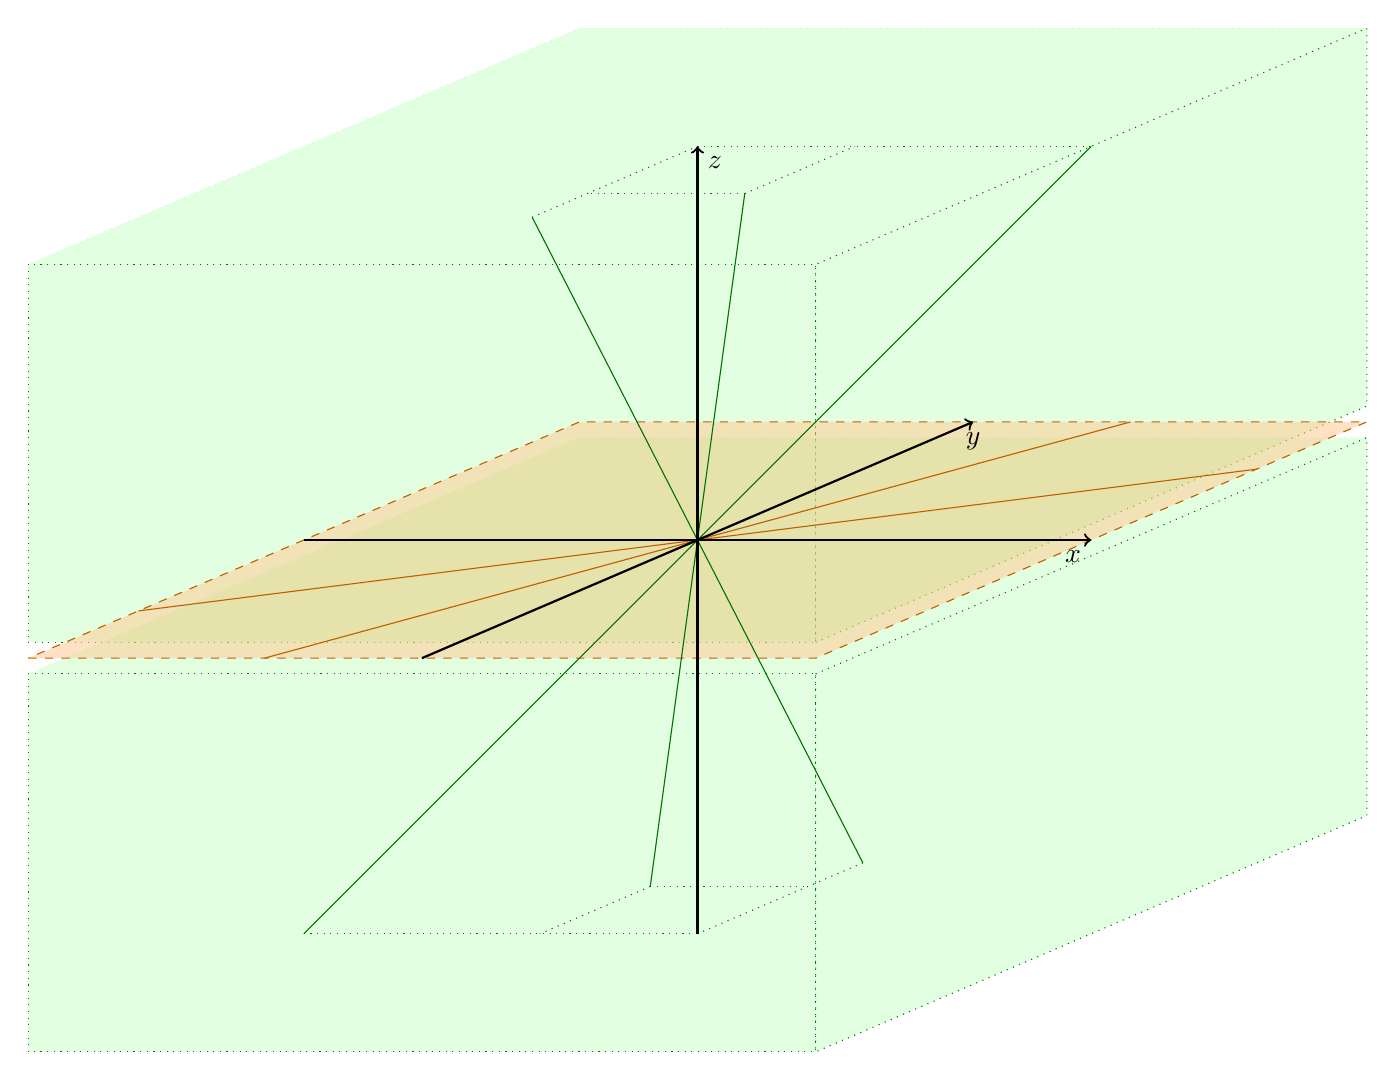
\begin{tikzpicture}[
		x={(1.0cm,0.0cm)},
		y={(0.7cm,0.3cm)},
		z={(0.0cm,1.0cm)}
	]

		% Upper space
		\draw [green!20, dotted, fill = green!45, fill opacity = 0.25] (-5,-5,5) -- (5,-5,5) -- (5,5,5) -- (-5,5,5) -- cycle;
		\draw [green!45!black, dotted, fill = green!45, fill opacity = 0.25] (-5,-5,0.2) -- (5,-5,0.2) -- (5,-5,5) -- (-5,-5,5) -- cycle;
		\draw [green!45!black, dotted, fill = green!45, fill opacity = 0.25] (5,-5,0.2) -- (5,5,0.2) -- (5,5,5) -- (5,-5,5) -- cycle;

		\draw [green!20, dotted, fill = green!45, fill opacity = 0.25] (-5,-5,-0.2) -- (5,-5,-0.2) -- (5,5,-0.2) -- (-5,5,-0.2) -- cycle;

		%plane 0
		\draw [orange!75!black, dashed, fill = orange!45, fill opacity = 0.50] (-5,-5,0) -- (5,-5,0) -- (5,5,0) -- (-5,5,0) -- cycle;

		% Lower space
		\draw [green!45!black, dotted, fill = green!45, fill opacity = 0.25] (-5,-5,-0.2) -- (5,-5,-0.2) -- (5,-5,-5) -- (-5,-5,-5) -- cycle;
		\draw [green!45!black, dotted, fill = green!45, fill opacity = 0.25] (5,-5,-0.2) -- (5,5,-0.2) -- (5,5,-5) -- (5,-5,-5) -- cycle;

		\draw [green!45!black] (-5,0,-5) -- (5,0,5);
		\draw [green!45!black, dotted] (-5,0,-5) -- (0,0,-5);
		\draw [green!45!black, dotted] (0,0,5) -- (5,0,5);

		\draw [green!45!black] (0,3,-5) -- (0,-3,5);
		\draw [green!45!black, dotted] (0,3,-5) -- (0,0,-5);
		\draw [green!45!black, dotted] (0,-3,5) -- (0,0,5);

		\draw [green!45!black] (-2,2,-5) -- (2,-2,5);
		\draw [green!45!black, dotted] (-2,2,-5) -- (-2,0,-5);
		\draw [green!45!black, dotted] (-2,2,-5) -- (0,2,-5);
		\draw [green!45!black, dotted] (2,-2,5) -- (2,0,5);
		\draw [green!45!black, dotted] (2,-2,5) -- (0,-2,5);

		\draw [orange!75!black] (-2,-5,0) -- (2,5,0);
		\draw [orange!75!black] (-5,-3,0) -- (5,3,0);


		\draw[thick,->] (-5,0,0) -- (5,0,0) node[anchor=north east]{$x$};;
		\draw[thick,->] (0,-5,0) -- (0,5,0) node[anchor=north]{$y$};;
		\draw[thick,->] (0,0,-5) -- (0,0,5) node[anchor=north west]{$z$};;
	\end{tikzpicture}

\end{document}
